\documentclass{beamer}
\usepackage{etex} % fixes new-dimension error
\usepackage{lmodern}
\usepackage[T1]{fontenc}
\newcommand{\norm}[1]{\left\lVert#1\right\rVert}
%%%%%%%%%%%%% Macros
\newcommand{\Ban}{\catfont{Ban}}
\newcommand{\Met}{\catfont{Met}}
\newcommand{\Shuff}{\mathrm{Sf}}
\newcommand{\Cats}{\catfont{Cat}}
\newcommand{\VCat}{\mathcal{V}\text{-}\Cats}
\newcommand{\VCatSy}{\mathcal{V}\text{-}\Cats_{\mathsf{sym}}}
\newcommand{\VCatSe}{\mathcal{V}\text{-}\Cats_{\mathsf{sep}}}
\newcommand{\VCatSS}{\mathcal{V}\text{-}\Cats_{\mathsf{sym,sep}}}
%%%% Categories
\newcommand{\catfont}[1]{\mathsf{#1}}
\newcommand{\cop}{\catfont{op}}
\newcommand{\Law}{\catfont{Law}}
\newcommand{\catV}{\catfont{V}}
\newcommand{\catX}{\catfont{X}}
\newcommand{\catC}{\catfont{C}}
\newcommand{\catD}{\catfont{D}}
\newcommand{\catA}{\catfont{A}}
\newcommand{\catB}{\catfont{B}}
\newcommand{\catI}{\catfont{I}}
\newcommand{\Set}{\catfont{Set}}
\newcommand{\Top}{\catfont{Top}}
\newcommand{\Pos}{\catfont{Pos}}
\newcommand{\Inj}{\catfont{Inj}}
\newcommand{\Det}{\catfont{RMhat}}
\newcommand{\CoAlg}[1]{\catfont{CoAlg}\left (#1 \right )}
\newcommand{\Mon}{\catfont{Mon}}
\newcommand{\Mnd}{\catfont{Mnd}(\catC)}
\newcommand{\SMnd}{\catfont{Mnd}(\Set)}
\newcommand{\CLat}{\catfont{CLat}}
\newcommand{\Stone}{\catfont{Stone}}
\newcommand{\Spectral}{\catfont{Spectral}}
\newcommand{\CompHaus}{\catfont{CompHaus}}
\newcommand{\Subs}[2]{\catfont{Sub}_{}}
\newcommand{\Cone}{\catfont{Cone}}
\newcommand{\StComp}{\catfont{StablyComp}}
\newcommand{\PosC}{\catfont{PosComp}}
\newcommand{\Haus}{\catfont{Haus}}
\newcommand{\Meas}{\catfont{Meas}}
\newcommand{\Ord}{\catfont{Ord}}
\newcommand{\EndoC}{[\catC,\catC]}
%% General functors
\newcommand{\funfont}[1]{#1}
\newcommand{\funF}{\funfont{F}}
\newcommand{\funU}{\funfont{U}}
\newcommand{\funG}{\funfont{G}}
\newcommand{\funT}{\funfont{T}}
\newcommand{\funI}{\funfont{I}}
%% Particular kinds of functors
\newcommand{\sfunfont}[1]{\mathrm{#1}}
\newcommand{\Pow}{\sfunfont{P}}
\newcommand{\Dist}{\sfunfont{D}}
\newcommand{\Maybe}{\sfunfont{M}}
\newcommand{\List}{\sfunfont{L}}
\newcommand{\UForg}{\sfunfont{U}}
\newcommand{\Forg}[1]{\sfunfont{U}_{#1}}
\newcommand{\Id}{\sfunfont{Id}}
\newcommand{\Vie}{\sfunfont{V}}
\newcommand{\Disc}{\funfont{D}}
\newcommand{\Weight}{\sfunfont{W}}
\newcommand{\homf}{\sfunfont{hom}}
\newcommand{\Yoneda}{\sfunfont{Y}}
%% Diagram functors
\newcommand{\Diag}{\mathscr{D}}
\newcommand{\KDiag}{\mathscr{K}}
\newcommand{\LDiag}{\mathscr{L}}
%% Monads
\newcommand{\monadfont}[1]{\mathbb{#1}}
\newcommand{\monadT}{\monadfont{T}}
\newcommand{\monadS}{\monadfont{S}}
\newcommand{\monadU}{\monadfont{U}}
\newcommand{\monadH}{\monadfont{H}}
\newcommand{\str}{\mathrm{str}}
%% Adjunctions
\newcommand\adjunct[2]{\xymatrix@=8ex{\ar@{}[r]|{\top}\ar@<1mm>@/^2mm/[r]^{{#2}}
& \ar@<1mm>@/^2mm/[l]^{{#1}}}}
\newcommand\adjunctop[2]{\xymatrix@=8ex{\ar@{}[r]|{\bot}\ar@<1mm>@/^2mm/[r]^{{#2}}
& \ar@<1mm>@/^2mm/[l]^{{#1}}}}
%% Retractions
\newcommand\retract[2]{\xymatrix@=8ex{\ar@{}[r]|{}\ar@<1mm>@/^2mm/@{^{(}->}[r]^{{#2}}
& \ar@<1mm>@/^2mm/@{->>}[l]^{{#1}}}}
%% Limits
\newcommand{\pv}[2]{\langle #1, #2 \rangle}
\newcommand{\limt}{\mathrm{lim}}
\newcommand{\pullbackcorner}[1][dr]{\save*!/#1+1.2pc/#1:(1,-1)@^{|-}\restore}
\newcommand{\pushoutcorner}[1][dr]{\save*!/#1-1.2pc/#1:(-1,1)@^{|-}\restore}
%% Colimits
\newcommand{\colim}{\mathrm{colim}}
\newcommand{\inl}{\mathrm{inl}}
\newcommand{\inr}{\mathrm{inr}}
%% Distributive categories
\newcommand{\distr}{\mathrm{dist}}
\newcommand{\undistr}{\mathrm{undist}}
%% Closedness
\newcommand{\curry}[1]{\mathrm{curry}{#1}}
\newcommand{\app}{\mathrm{app}}
%% Misc. operations
\newcommand{\const}[1]{\underline{#1}}
\newcommand{\comp}{\cdot}
\newcommand{\id}{\mathrm{id}}
%% Factorisations
\newcommand{\EClass}{E}
\newcommand{\MClass}{M}
\newcommand{\MConeClass}{\mathcal{M}}
%%%%%%%%%%%%%%%% End of Categorical Stuff

%%%% Misc
%% Operations
\newcommand{\blank}{\, - \,}
\newcommand{\sem}[1]{\llbracket #1 \rrbracket}
\newcommand{\closure}[1]{\overline{#1}}
\DeclareMathOperator{\img}{\mathrm{im}}
\DeclareMathOperator{\dom}{\mathrm{dom}}
\DeclareMathOperator{\codom}{\mathrm{codom}}
%% Sets of numbers
\newcommand{\Nats}{\mathbb{N}}
\newcommand{\Reals}{\mathbb{R}}
\newcommand{\Rz}{\Reals_{\geq 0}}
\newcommand{\Complex}{\mathbb{C}}
%% Writing
\newcommand{\cf}{\emph{cf.}}
\newcommand{\ie}{\emph{i.e.}}
\newcommand{\eg}{\emph{e.g.}}
\newcommand{\df}[1]{\emph{\textbf{#1}}}
%%%%%%%%%%%%%%%% End of Misc

%%%% Programming Stuff
%% Types
\newcommand{\typefont}[1]{\mathbb{#1}}
\newcommand{\typeOne}{1}
\newcommand{\typeTwo}{2}
\newcommand{\typeA}{\typefont{A}}
\newcommand{\typeX}{\typefont{X}}
\newcommand{\typeB}{\typefont{B}}
\newcommand{\typeC}{\typefont{C}}
\newcommand{\typeV}{\typefont{V}}
\newcommand{\typeD}{\typefont{D}}
\newcommand{\typeI}{\typefont{I}}
%% RuleName
\newcommand{\rulename}[1]{(\mathrm{#1})}
%% Sequents
\newcommand{\jud}{\vdash}
\newcommand{\vljud}{\rhd}
\newcommand{\cojud}{\vdash_{\co}}
\newcommand{\vl}{\mathtt{v}}
\newcommand{\co}{\mathtt{c}}
% Program font
\newcommand{\prog}[1]{\mathtt{#1}}
\newcommand{\pseq}[3]{#1 \leftarrow #2; #3}
\newcommand{\ppm}[4]{(#1,#2) \leftarrow #3; #4}
\newcommand{\pinl}[1]{\prog{inl}(#1)}
\newcommand{\pinr}[1]{\prog{inr}(#1)}
\newcommand{\pcase}[4]{\prog{ case } #1 \prog{ of } \pinl{#2} \Rightarrow #3 ; \pinr{#2} \Rightarrow #4}
%% Sets of terms
\newcommand{\ValuesBP}[2]{\mathsf{Values}(#1, #2)}
\newcommand{\TermsBP}[2]{\mathsf{Terms}(#1, #2)}
\newcommand{\closValP}[1]{\ValuesBP{\emptyset}{#1}}
\newcommand{\closTermP}[1]{\TermsBP{\emptyset}{#1}}
\newcommand{\closVal}{\closValP{\typeA}}
\newcommand{\closTerm}{\closTermP{\typeA}}
%% Contextual equivalence
\newcommand{\ctxeq}{\equiv_{\prog{ctx}}}
%%%% End of Programming Stuff

%-------------- template --------------------------------------------------
\usetheme{metropolis}
\metroset{block=fill}
%\usetheme{Boadilla}
% Configuring the foot line
\setbeamertemplate{footline}
{
  \leavevmode%
  \hbox{%
  \begin{beamercolorbox}[wd=.4\paperwidth,ht=2.25ex,dp=1ex,center]{author in head/foot}%
    \usebeamerfont{author in head/foot}\insertshortauthor
  \end{beamercolorbox}%
  \begin{beamercolorbox}[wd=.5\paperwidth,ht=2.25ex,dp=1ex,center]{title in head/foot}%
    \usebeamerfont{title in head/foot}\insertsection
  \end{beamercolorbox}%
  \begin{beamercolorbox}[wd=.1\paperwidth,ht=2.25ex,dp=1ex,right]{date in head/foot}%
    \insertframenumber{} / \inserttotalframenumber\hspace*{2ex} 
  \end{beamercolorbox}}%
  \vskip0pt%
}
% No configuration symbols
\setbeamertemplate{navigation symbols}{}
%--------------- packages -------------------------------------------------
\usepackage{graphicx,amsmath}
\usepackage{stmaryrd} % cf. interleave
\usepackage{booktabs}
\usepackage{amscd}
\usepackage{multicol}
\usepackage[absolute,overlay]{textpos}
\usepackage{alltt}
\usepackage{proof}
\usepackage{subcaption}
\usepackage{tikz}
\usepackage{tikz-cd}
\usepackage[new]{old-arrows}
\usepackage[all]{xy}
\usepackage{pgfplots}
\usepackage{textcomp}
\usetikzlibrary{arrows.meta, calc, fit, tikzmark}
\usepackage{pstricks,pst-node,pst-text,pst-3d}

% context
\AtBeginSection[]
{
    \begin{frame}
        \frametitle{Table of Contents}
        \tableofcontents[currentsection]
    \end{frame}
}

\author[Renato Neves]{Renato Neves}

% logos of institutions
\titlegraphic{
  \begin{textblock*}{5cm}(6.7cm,7.45cm)
     
\includegraphics[scale=0.06]{logos/uminho.png}\hspace*{.85cm}~%
  \end{textblock*}
  \begin{textblock*}{5cm}(9.4cm,7.42cm)
    
\includegraphics[scale=0.50]{logos/haslab.pdf}
  \end{textblock*}
}

% No date
\date{}

\begin{document}

\title{Quantum Computation}

\frame[plain]{\titlepage}

\section{The context}

\begin{frame}{Context}

  Quantum Computing is coming of age

  \dots\ moving from a potential far-future technology
  to a stage where prototypes become available and
  \alert{major investments} arise
  \begin{itemize}
  \item Companies (IBM, Google, Microsoft, and Intel)
  \item Public investment (UK, Sweden, Canada, Australia, Portugal)
  \item EU Flagship initiative with a 10 year timespan and an
  estimated budget of over one billion euros
  \end{itemize}
\end{frame}

\begin{frame}{Why the big interest?}
        
  A strategic use of quantum mechanics potentially provides remarkable speedups
  to hard \alert{computational} problems

  \begin{itemize}
  \item Cryptographic mechanisms
  \item Molecule simulation and weather prediction
  \item Processing of large data
  \end{itemize}

  \dots\ and also more secure \alert{communication protocols}
\end{frame}

\begin{frame}{Why the big interest? (A concrete example)}

  Cryptographic schemes often assume that factoring large integers is
  computationally intractable
  
  In 1994 Peter Shor presented a quantum \alert{algorithm} for factoring
  integers that runs in \dots\ \alert{polynomial time} 

  \vfill

  \begin{textblock*}{4cm}(8cm,5.35cm)
    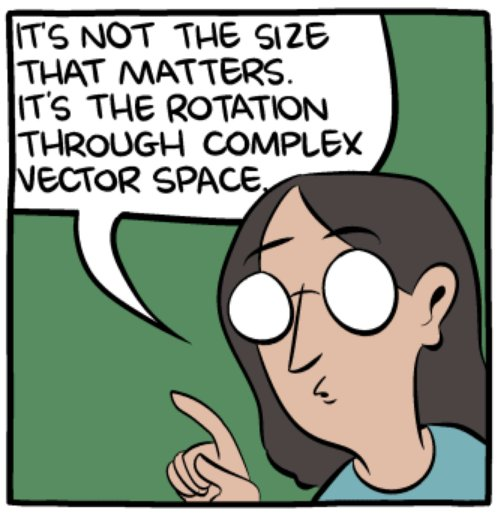
\includegraphics[scale=0.2]{images/size.jpg}
    \tiny{smbc-comics}
  \end{textblock*}

\end{frame}

\begin{frame}{Why the big interest? (Concrete example II)}

  Transmission of information via \alert{\underline{superposition}} and
  \alert{\underline{entanglement}}


  Eavesdropping becomes detectable 
  \vfill
  \begin{textblock*}{3.5cm}(8.7cm,5.5cm)
    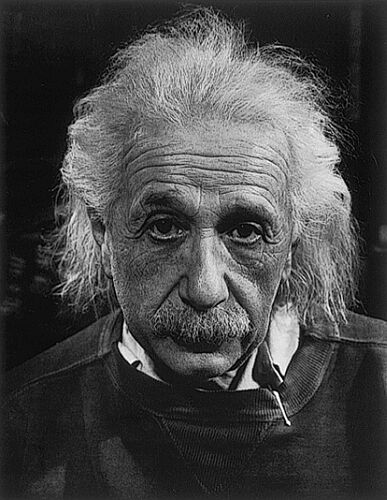
\includegraphics[scale=0.20]{images/einstein.jpg}
  \end{textblock*}

\end{frame}

\section{A brief history of Quantum Computation}

\begin{frame}{The Modern Reincarnation of Computing Science}

  \begin{minipage}[0.3\textheight]{\textwidth}
  \begin{columns}[c]
  \begin{column}{0.7\textwidth}
          On Computable Numbers, with an Application to the 
          \tikzmark{z1}\emph{Entscheidungsproblem}\tikzmark{z2}, 1936
  \end{column}
  \begin{column}{0.3\textwidth}
    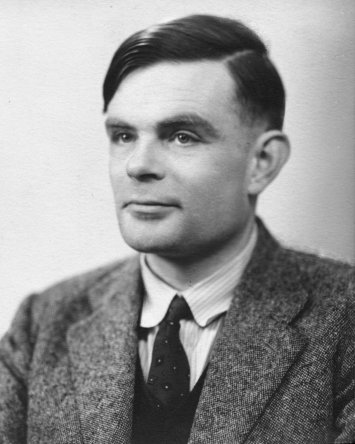
\includegraphics[scale=2]{images/turing.jpg}
  \end{column}
  \end{columns}
  \end{minipage}

  \begin{tikzpicture}[overlay,remember picture,
       box/.style = {rounded corners},
       pin edge={-Stealth,thick, red}]
       \coordinate (z1) at ($({pic cs:z1})+(+0.5ex, 1.5ex)$);
       \coordinate (z2) at ($({pic cs:z2})+(-0.5ex,-0.5ex)$);
       \node[semitransparent, 
             fit=(z1) (z2),
             pin=below:\tiny{Homework: See/read 
             \emph{The Hitchhiker's Guide to the Galaxy}}]  {};
   \end{tikzpicture}

\end{frame}

\begin{frame}{A Case for Quantum Computing}

  \begin{minipage}[0.3\textheight]{\textwidth}
  \begin{columns}[c]
  \begin{column}{0.6\textwidth}
          Simulating Physics with Computers, 1982
  \end{column}
  \begin{column}{0.4\textwidth}
    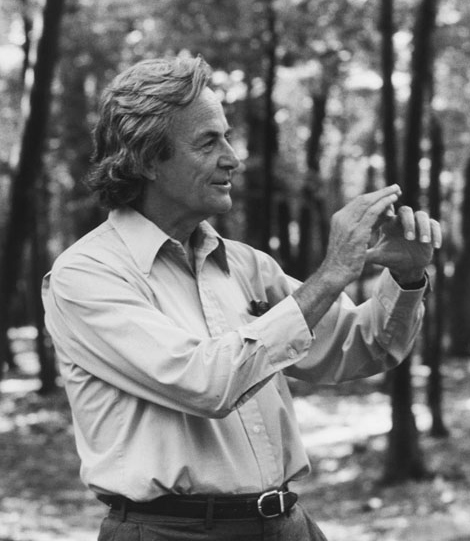
\includegraphics[scale=1]{images/feynman.jpg}
  \end{column}
  \end{columns}
  \end{minipage}

  \vfill
  \scriptsize{
          "\dots \emph{because nature isn't
                  classical, dammit, and if you want to make a simulation of nature, you'd
                  better make it quantum mechanical, and by golly it's a wonderful problem,
                  because it doesn't look so easy.}"
  }

\end{frame}

\begin{frame}{Quantum Computational Model}

  \begin{minipage}[0.3\textheight]{\textwidth}
  \begin{columns}[c]
  \begin{column}{0.6\textwidth}
        Quantum theory, the Church-Turing principle and the universal quantum computer,
        1985
  \end{column}
  \begin{column}{0.4\textwidth}
    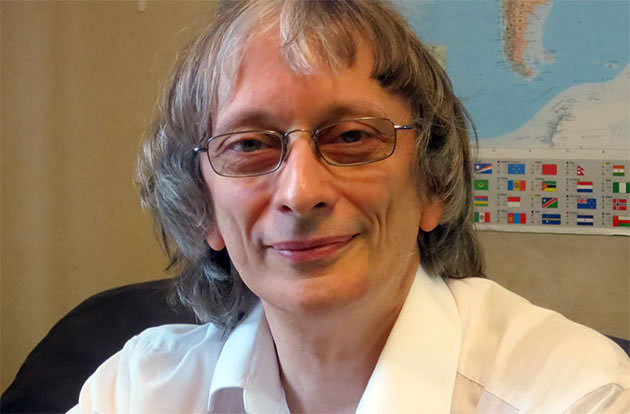
\includegraphics[scale=0.2]{images/deutsch.jpg}
  \end{column}
  \end{columns}
  \end{minipage}

  \vfill
  \scriptsize{
        Quantum computability and computational model: first example of a quantum
        algorithm that is remarkably faster than any possible classical one
  }

\end{frame}

\begin{frame}{The Field of Quantum Computation}
  \begin{columns}[c]
  \begin{column}{0.33\textwidth}
          \centering
          \small{Computability} \\
          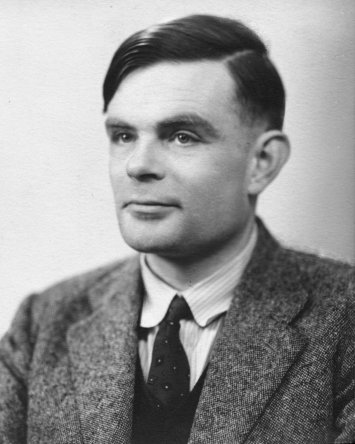
\includegraphics[height=2.4cm]{images/turing.jpg}
  \end{column}
  \begin{column}{0.33\textwidth}
          \centering
          \small{Quantum Computing} \\
          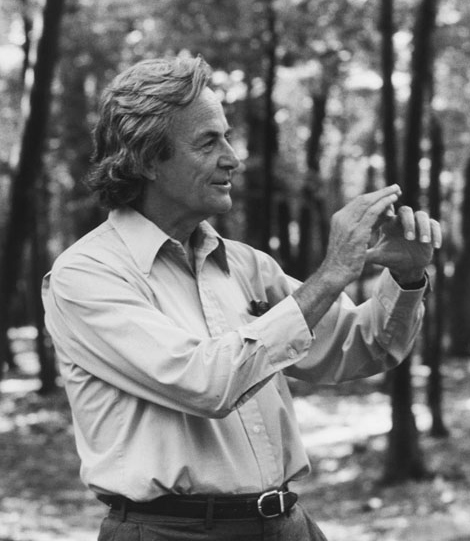
\includegraphics[height=2.4cm]{images/feynman.jpg}
  \end{column}
  \begin{column}{0.4\textwidth}
          \centering
          \small{Quantum Computability} \\
          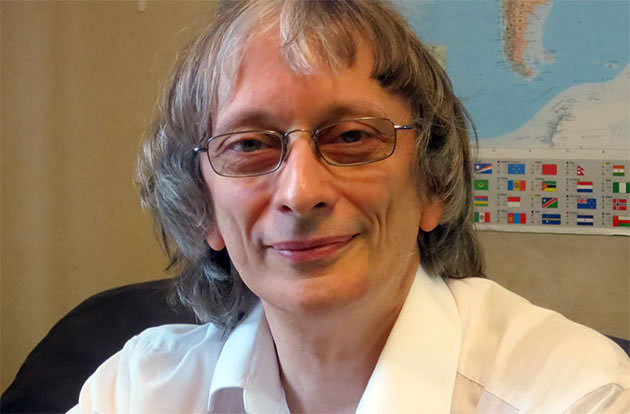
\includegraphics[height=2.4cm]{images/deutsch.jpg}
  \end{column}
  \end{columns}

  \vfill
  \dots and of course many others 
\end{frame}

\section{Currently \dots}

\begin{frame}{The Second Quantum Revolution}

        Viability of quantum computing demonstrated in problems difficult to
        handle classically 

        \begin{itemize}
        \item Google's Sycamore, 2019
        \item Zuchongzhi, 2021
        \end{itemize}

\end{frame}

\begin{frame}{However \dots}

        The quantum race has just started
        
        \begin{itemize}
                \item current quantum computers are \alert{unreliable}
                        for performing actually useful computational
                        tasks
                \item difficult to anticipate 
                        their  evolution and future applications
                \item commercial/military potential in the short term (5 to 10 yrs) 
                        is still highly debatable
        \end{itemize}
\end{frame}

\begin{frame}{In the Short Term}
  \begin{minipage}[0.3\textheight]{\textwidth}
  \begin{columns}[c]
  \begin{column}{0.7\textwidth}
        Quantum advantage with the \alert{Noisy Intermediate-Scale Quantum}
        (NISQ) computational model 
        \begin{itemize}
                \item the quantum device as a coprocessor
                \item typically accessed as a service over the cloud 
        \end{itemize}
  \end{column}
  \begin{column}{0.3\textwidth}
        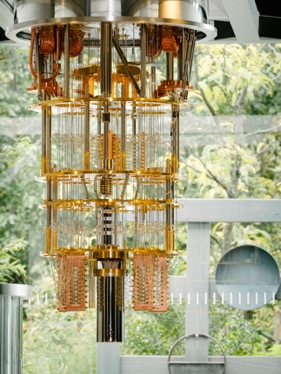
\includegraphics[height=3.5cm]{./images/qc.jpg} 
  \end{column}
  \end{columns}
  \end{minipage}
\end{frame}

\section{The course}

\begin{frame}{Learning Outcomes}

On successful completion of the course students should be able to,

\begin{itemize}
\item understand basic concepts of computability and computational complexity;
\item understand basic concepts and techniques in quantum algorithmics;
\item design and analyse quantum algorithms;
\item implement and run quantum algorithms in the \alert{\textsc{Qiskit}} 
        open-source software development kit.
\end{itemize}

\end{frame}

\begin{frame}{Course Information and Pragmatics}

\begin{block}{Refer to the course's website at}
\begin{center}
        \url{lmf.di.uminho.pt/quantum-computation-2223/}
\end{center}
\end{block}

\end{frame}

\begin{frame}[plain]

\end{frame}

\end{document}
